\documentclass[10pt]{standalone}

\usepackage{tikz}
\usepackage{pgfplots}
\usepackage[cmex10]{amsmath}
\usepackage{amsfonts}
 \pgfplotsset{compat=1.12}
%\usepgfplotslibrary{polar}

\begin{document}

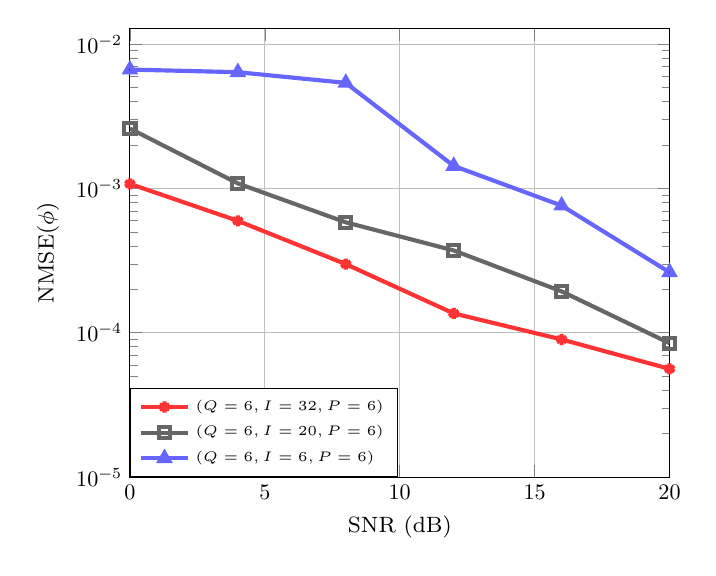
\begin{tikzpicture}

  \begin{axis}[%
ymode = log,
%scale only axis,
%separate axis lines,
%every outer x axis line/.append style={black},
%every x tick label/.append style={font=\color{black}},
every tick label/.append style={scale=0.8},
xmin=0,
xmax=20,
xlabel={\footnotesize{SNR (dB)}},
%xmajorgrids,
%every outer y axis line/.append style={black},
%every y tick label/.append style={font=\color{black}},
ylabel={ \footnotesize{NMSE($\phi$)}},
ymin = 0.00001,
%title = Channel frequency response between $\mathbf{H}(2,1)$,
%ymajorgrids,
grid,
%axis background/.style={fill=white},
legend style={at={(0,0)},anchor=south west,legend cell align=left,align=left,draw=black,font=\fontsize{4}{4}\selectfont}
]

%%%%%%%%%%%%%%%%%%%%%%%%% M=8 %%%%%%%%%%%%%%%%%%%%%%%%%%%%%%%%%%%%%%%%%%%%%%%%%


\addplot [color=red!80,solid,mark=asterisk,mark options={solid},line width=1.5pt,mark size=2pt]
  table[row sep=crcr]{%
0 0.00107523 \\
4 0.00059626 \\
8 0.00029883 \\
12 0.00013613 \\
16 0.00008986 \\
20 0.000056222 \\
};
\addlegendentry{$(Q=6,I=32,P=6)$}; 


\addplot [color=black!60,solid,mark=square,mark options={solid},line width=1.5pt,mark size=2pt]
   table[row sep=crcr]{%
0 0.0025996 \\
4 0.00108247 \\
8 0.00058217 \\
12 0.00037176 \\
16 0.0001935 \\
20 0.0000847 \\
 };
\addlegendentry{$(Q=6,I=20,P=6)$};

\addplot [color=blue!60,solid,mark=triangle,mark options={solid},line width=1.5pt,mark size=2pt]
  table[row sep=crcr]{%
0 0.0066585 \\
4 0.0063854 \\
8 0.0053848 \\
12 0.0014317 \\
16 0.00076007 \\
20 0.00026234 \\
};
\addlegendentry{$(Q=6,I=6,P=6)$};

% \addplot [color=green!80,solid,mark=diamond,mark options={solid},line width=1.5pt,mark size=2pt]
%   table[row sep=crcr]{%

% };
% \addlegendentry{$(Q=6,I=2,P=6)$};

\end{axis}
\end{tikzpicture}
\end{document}

%%% Local Variables:
%%% mode: latex
%%% TeX-master: t
%%% End:
